\documentclass{article}
\usepackage[utf8]{inputenc}
\usepackage[english]{babel}
\usepackage[font=small,labelfont=bf]{caption}
\usepackage{geometry}
\usepackage{natbib}
\usepackage{pxfonts}
\usepackage{graphicx}
\usepackage{newfloat}
\usepackage{setspace}
%\doublespacing

\newcommand{\argmax}{\mathop{\mathrm{argmax}}\limits}

\title{\textit{Supporting Information for}: How is experience transformed into memory?}
\author{Andrew C. Heusser, Paxton C. Fitzpatrick, and Jeremy R. Manning\\Department of Psychological and Brain Sciences\\Dartmouth College, Hanover, NH 03755, USA\\Corresponding author: jeremy.r.manning@dartmouth.edu}

\bibliographystyle{apa}

\begin{document}
\maketitle

\setcounter{equation}{0}
\setcounter{figure}{0}
\setcounter{table}{0}
\setcounter{page}{1}
\setcounter{section}{0}
\makeatletter
\renewcommand{\theequation}{S\arabic{equation}}
\renewcommand{\thefigure}{S\arabic{figure}}
\renewcommand{\bibnumfmt}[1]{[S#1]}
\renewcommand{\citenumfont}[1]{S#1}


\section*{Overview}
This document provides additional details about the methods we used in the main text.  We also include some additional analyses referenced in the main text.

\section*{Additional details about topic modeling methods and results}
\subsection*{Optimizing topic model parameters}
In order to create accurate video and recall models, we used an optimization method that was driven by our ability to explain hand-annotated memory performance metrics collected by \cite{ChenEtal17}.  Specifically, we used a grid search to compute the $\omega$ (video sliding window duration, in scenes), $\rho$ (recall sliding window duration, in sentences), and $K$ (number of topics) that satisfied
\[
\argmax_{\omega, \rho, K} \left[\mathrm{corr}\left(\mathrm{corr}\left(\mu\left(\omega, \rho, K\right), \nu\left(\omega, \rho, K\right)\right), \theta\right)\right],
\]
where $\mathrm{corr}(\mu, \nu)$ is the per-participant correlation between the upper triangles of the temporal correlation matrices of the video ($\mu$) and recall ($\nu$) trajectory, and $\theta$ is the per-participant hand-annotated memory performance.  We searched over a grid of pre-specified values for each of these parameters; the resulting correlations are displayed in Figure~\ref{fig:paramsearch}.  The optimal parameters were $\omega = 50$, $\rho = 10$, and $K = 100$.


\begin{figure}[p!]
\centering
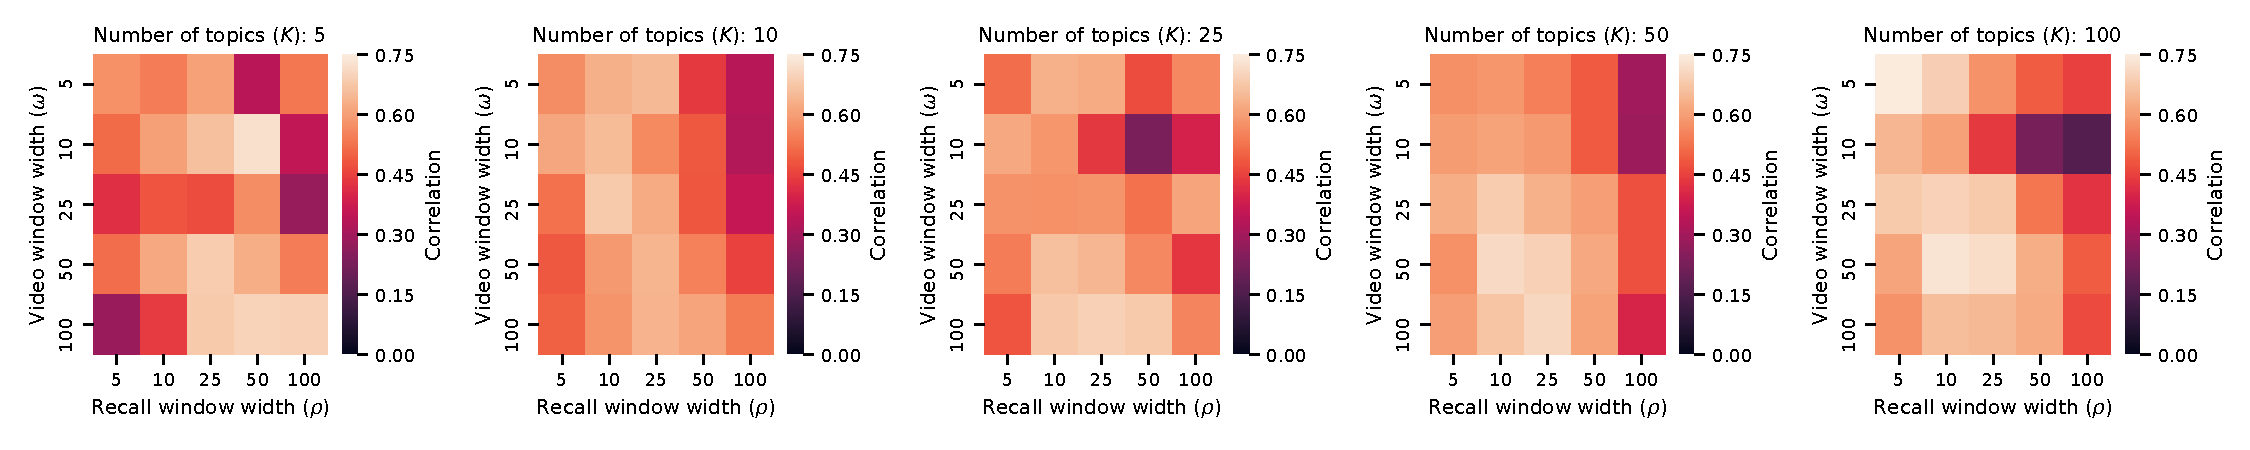
\includegraphics[width=1\textwidth]{figs/parameter_search}
\caption{\small \textbf{Optimizing topic model parameters.}  We performed a grid search over video sliding window length ($\omega \in \{5, 10, 25, 50, 100 \}$), recall sliding window length ($\rho \in \{5, 10, 25, 50, 100 \}$, and number of topics ($K \in \{5, 10, 25, 50, 100 \}$.  The reported correlations are between per-subject video-recall trajectory correlations and per-subject hand-annotated memory performance ratings.}
\label{fig:paramsearch}
\end{figure}

The optimized model converged on 27 unique topics that were assigned non-zero weights over the course of the video.  We provide a list of the top ten highest-weighted words from each topic in Figure~\ref{fig:topics}.

\begin{figure}[p!]
\centering
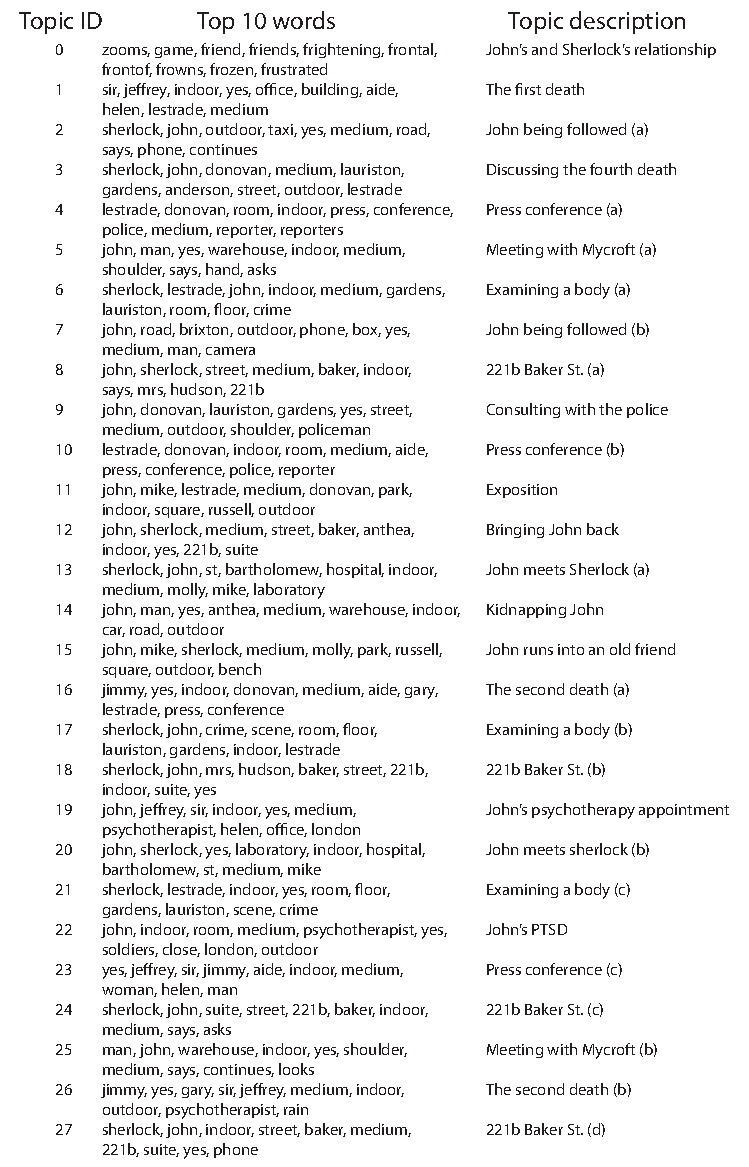
\includegraphics[width=0.75\textwidth]{figs/topic_words}
\caption{\small \textbf{Topics discovered in \textit{Sherlock}.} We applied a topic model to hand-annotated information about 1000 scenes spanning the 45 minute episode.  We identified 27 unique topics with non-zero weights (we used $K=100$ topics to fit the model).  Each topic comprises a distribution of weights over all words in the vocabulary.  For each topic, we show the words with the 10 largest weights, along with a suggested description of the topic.}
\label{fig:topics}
\end{figure}


\subsection*{Feature importance analyses}
To determine the contribution of each feature to the structure of the video topic proportions, we conducted a ``leave one out'' analysis.  Specifically, we compared the original video topic trajectory (created using all hand-annotated features from the 1000 hand-annotated scenes spanning the \textit{Sherlock} episode; see \textit{Methods} for a full list of features) with video trajectories created using all but one type of feature.  We created temporal correlation matrices for each trajectory (using the topic proportions matrices) and correlated the upper triangles of each impoverished trajectory with the original feature-complete trajectory.  Observing a lower correlation between an impoverished trajectory (holding out a particular feature) and the feature-complete trajectory would suggest that the given feature played a more prominent role in shaping the structure of the feature-complete trajectory.  We found that hand-annotated narrative details provided the most structure to the feature-complete trajectory, whereas transcriptions of onscreen text provided the least structure (Fig.~\ref{fig:feature-importance}A).

\begin{figure}[p!]
\centering
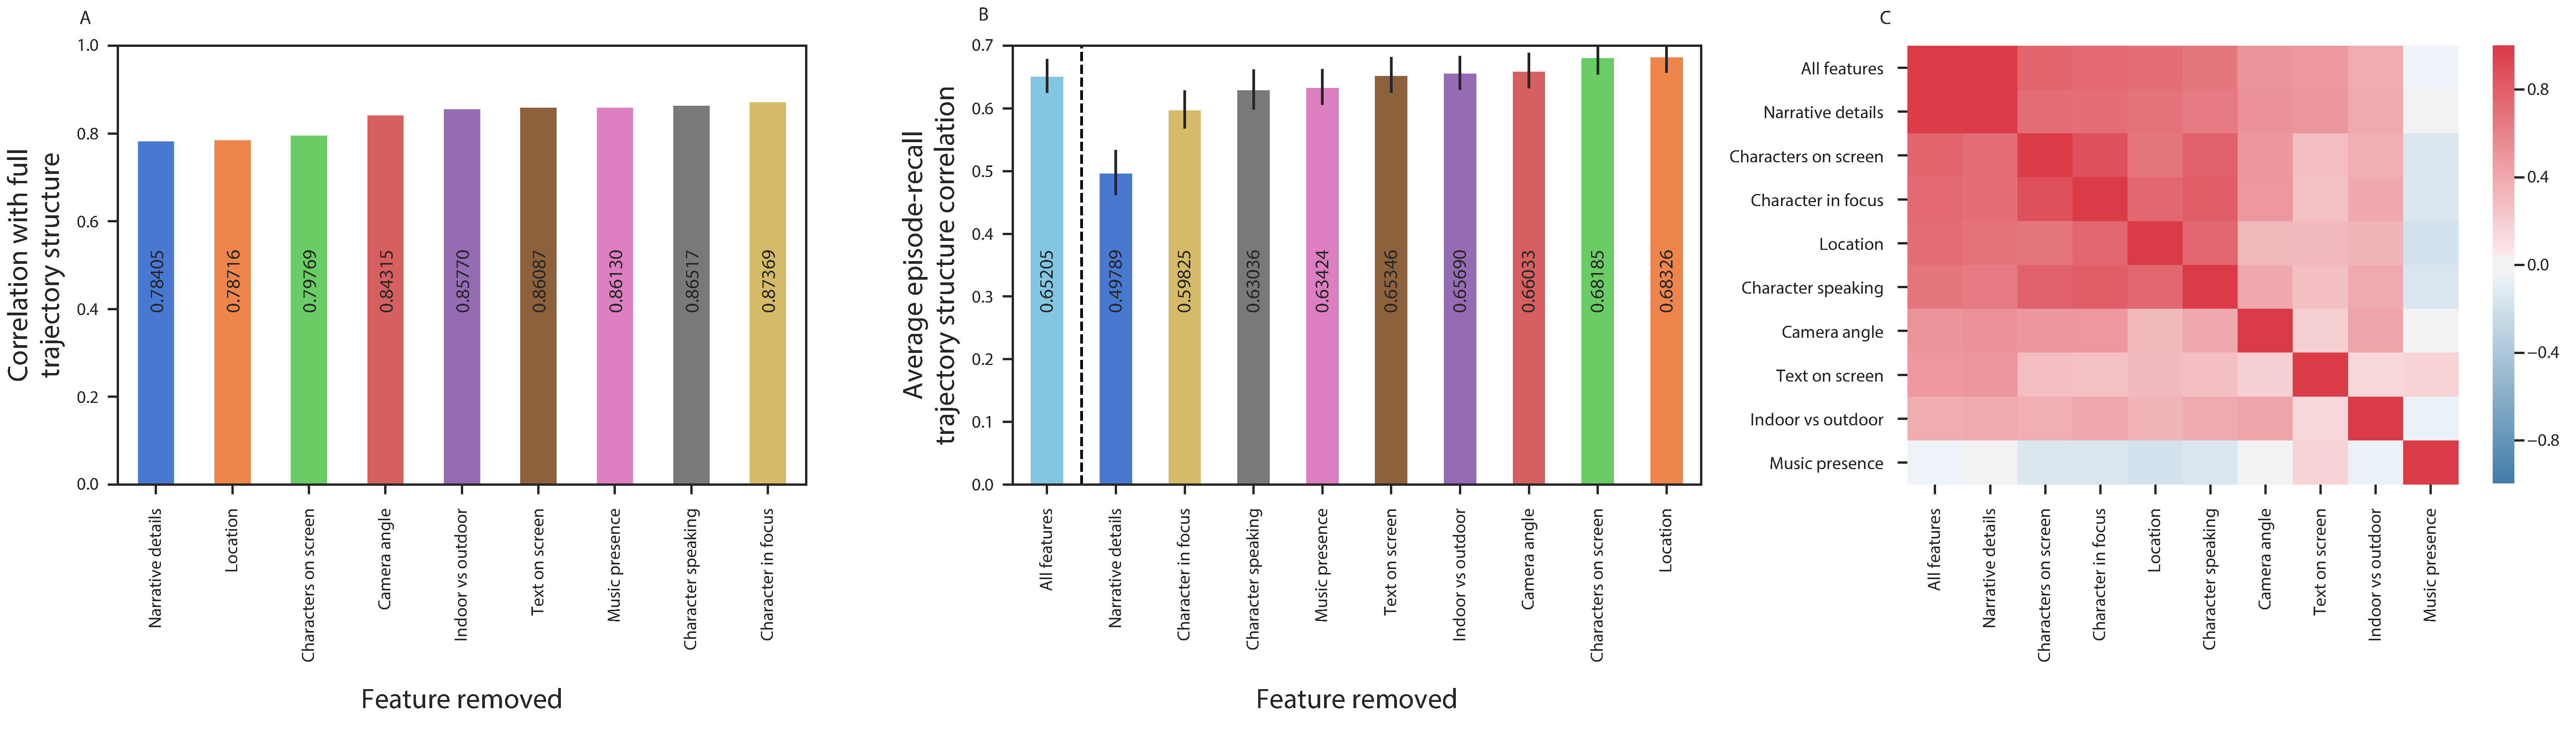
\includegraphics[width=1\textwidth]{figs/feature_value}
\caption{\small \textbf{Feature importance analysis.} \textbf{A.} Contributions of each feature type to the structure of the video trajectory. The bar heights reflect the correlation between the video trajectory computed using all features with a video trajectory computed using all features except the indicated feature.  (Lower bars reflect features that contribute more substantially to the video trajectory's shape.) \textbf{B.} Which features are preserved during recall?  The bar heights reflect the (average) across-participant correlations between the video and recall trajectories.  Error bars denote bootstrap-estimated standard error of the mean.  \textbf{C.} Feature correlation matrix.  Each entry displays the correlation between video topic trajectories created using only the indicated (row/column) features.}
\label{fig:feature-importance}
\end{figure}

We also carried out an analysis of which annotated features tended to shape aspects of the video topic trajectory that were preserved in participants' recalls.  Specifically, we computed the timepoint-by-timepoint correlation matrix of the video topic trajectory, and correlated its upper triangle with that of the timepoint-by-timepoint correlation matrices of each participant's recall topic trajectory (resampled using linear interpolation to have the same number of timepoints as the video trajectory).  This yielded a single correlation coefficient for each participant.  We then repeated this analysis with each annotated feature held out in turn.  Observing a lower correlation between the video and recall trajectories (when a given feature was held out) would indicate that the feature tends to be preserved in participants' recalls.  We found that hand-annotated narrative details were the most preserved type of feature, whereas information about the camera angle tended not to influence participants' recalls (Fig.~\ref{fig:feature-importance}B).

Next, we wondered how the different types of features might relate.  For example, knowing which characters are on screen during a given scene may also provide information about which characters are speaking.  We computed video topic trajectories for each feature in turn, and then compared the temporal correlation matrices of all pairs of features.  This provided additional confirmation that the shape of the full trajectory (including all types of features) was largely driven by narrative details.  We also found that character-driven features (characters on screen, characters speaking, and characters in focus) were strongly correlated.  Other details, such as the presence or absence of music, led to very different topic trajectories (Fig.~\ref{fig:feature-importance}C).


% \section*{Additional analyses of memory performance}

% \subsection*{Naturalistic extensions of classic list-learning analyses}
% In traditional list-learning experiments, participants view a list of items (e.g., words) and then recall the items later.  Our video-recall event matching approach affords us the ability to analyze memory in a similar way. The video and recall events can be treated analogously to studied and recalled ``items'' in a list-learning study.  We can then extend classic analyses of memory performance and dynamics (originally designed for list-learning experiments) to the more naturalistic video recall task used in our study.

% Perhaps the simplest and most widely used measure of memory performance is \textit{accuracy}-- i.e., the proportion of studied (experienced) items (in this case, the 34 video events) that the participant later remembered.  \cite{ChenEtal17} developed a human rating system whereby the quality of each participant's memory was evaluated by an independent rater.  We found a strong across-participants correlation between these independant ratings and the overall number of events that our HMM approach identified in participants' recalls (Pearson's $r(15) = 0.67, p = 0.003$).

% As described below, we next considered three more nuanced measures of the memory performance and dynamics that are typically associated with list-learning studies.  We also provide a software package, \texttt{Quail}, for carrying out these analyses~\citep{HeusEtal17b}.

% \begin{figure}[p!]
% \centering
% 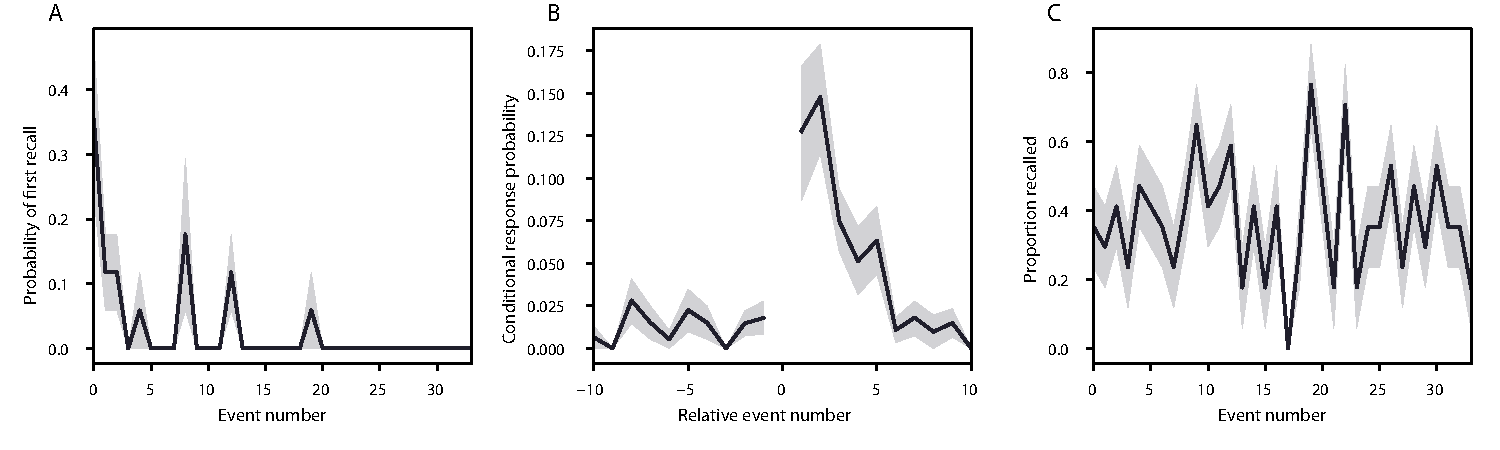
\includegraphics[width=1\textwidth]{figs/list_learning}
% \caption{\small \textbf{Naturalistic extensions of classic list-learning memory analyses.} \textbf{A.} The probability of first recall as a function of the serial position of the event in the video. \textbf{B}.  The probability of recalling each event, conditioned on having most recently recalled the event \textit{lag} events away in the video.  \textbf{C.} The proportion of participants who recalled each event, as a function of the serial position of the events in the video.  All panels: error bars denote bootstrap-estimated standard error of the mean.}
% \label{fig:list-learning}
% \end{figure}

% \paragraph{Probability of first recall (PFR).}  PFR curves~\citep{WelcBurn24, PostPhil65, AtkiShif68} reflect the probability that an item will be recalled first as a function of its serial position during encoding. To carry out this analysis, we initialized a number-of-participants (17) by number-of-video-events (34) matrix of zeros. Then for each participant, we found the index of the video event that was recalled first (i.e., the video event whose topic vector was most strongly correlated with that of the first recall event) and filled in that index in the matrix with a 1.  Finally, we averaged over the rows of the matrix, resulting in a 1 by 34 array representing the proportion of participants that recalled an event first, as a function of the order of the event's appearance in the video (Fig.~\ref{fig:list-learning}A).

% \paragraph{Lag conditional probability curve (lag-CRP).} The lag-CRP curve~\citep{Kaha96} reflects the probability of recalling a given event after the just-recalled event, as a function of their relative positions (or \textit{lag}).  In other words, a lag of 1 indicates that a recalled event came immediately after the previously recalled event in the video, and a lag of -3 indicates that a recalled event came 3 events before the previously recalled event.  For each recall transition (following the first recall), we computed the lag between the current recall event and the next recall event, normalizing by the total number of possible transitions.  This yielded a number-of-participants (17) by number-of-lags (-33 to +33; 67 lags total) matrix. We averaged over the rows of this matrix to obtain a group-averaged lag-CRP curve (Fig.~\ref{fig:list-learning}B).

% \paragraph{Serial position curve (SPC).} SPCs~\citep{Murd62a} reflect the proportion of participants that remember each item as a function of their serial position during encoding. We initialized a number-of-participants (17) by number-of-video-events (34) matrix of zeros. Then, for each recalled event, for each participant, we found the index of the video event that the recalled event most closely matched (via the correlation between the events' topic vectors) and entered a 1 into that position in the matrix (i.e., for the given participant and event). This resulted in a matrix whose entries indicated whether or not each event was recalled by each participant (depending on whether the corresponding entires were set to one or zero).  Finally, we averaged over the rows of the matrix to yield a 1 by 34 array representing the proportion of participants that recalled each event as a function of the order of the event's appearance in the video (Fig.~\ref{fig:list-learning}C).

% \paragraph{Temporal clustering scores.} Temporal clustering refers to the extent to which participants group their recall responses according to encoding position~\citep{PolyEtal09}. For instance, if a participant recalled the video events in the exact order they occurred (or in exact reverse order), this would yield a score of 1.  If a participant recalled the events in random order, this would yield an expected score of 0.5.  For each recall event transition (and separately for each participant), we sorted all not-yet-recalled events according to their absolute lag (i.e., distance away in the video).  We then computed the percentile rank of the next event the participant recalled.  We averaged these percentile ranks across all of the participant's recalls to obtain a single temporal clustering score for the participant (mean: 0.808, SEM: 0.022).  Overall, we found that participants with higher temporal clustering scores also tended to recall more events (Pearson's $r(15) = 0.62, p = 0.007$).

% \paragraph{Semantic clustering scores.} Semantic clustering measures the extent to which participants clustered their recall responses according to semantic similarity~\citep{PolyEtal09}. Here, we used the topic vectors for each event as a proxy for its semantic content. Thus, the similarity between the semantic content for two events can be computed by correlating their respective topic vectors.  For each recall event transition, we sorted all not-yet-recalled events according to how correlated the topic vector \textit{of the closest-matching video event} was to the topic vector of the closest-matching video event to the just-recalled event.  We then computed the percentile rank of the observed next recall.  We averaged these percentile ranks across all of the participant's recalls to obtain a single semantic clustering score for the participant (mean: 0.813, SEM: 0.022).  We found that participants who exhibited stronger semantic clustering scores overall remembered more video events (Pearson's $r(15) = 0.55, p = 0.02$).

% \subsection*{Novel memory measures afforded by our framework}
% To quantify the similarity between the video topic trajectory and individual recall topic trajectories, we considered several novel metrics.  First, we tested whether each participant's recall trajectory matched the video trajectory in a general sense. For each participant we filtered the video trajectory to only include the events that the participant remembered.  We then computed the root mean squared difference (RMSD) between the remaining video events and the (closest-matching) recalled events.  For example, if the topic vectors for a participant's recall event topic vectors matched the corresponding video event topic vectors exactly (and in order), the expected RMSD for those events would be 0.  However, if the participant's recall events did not perfectly match the video events, or if they were out of order, then the RMSD would be greater than 0.  To assess the significance of the match between the video and recall trajectories, we carried out a permutation procedure whereby, for each of 10000 repetitions, we circularly shifted the recall trajectories (in time) by a random amount and then re-computed the RMSD each time.  This yielded a distribution of ``null'' RMSD values for each participant.  The observed RMSD values reached significance (i.e., $p < 0.05$, reflecting that more than 95\% of the null RMSD values were greater than the observed RMSD value) for nine of the participants (3, 4, 8--13, and 17).  (For the remaining participants this test yielded $0.05 \leq p < 0.25$.)  The observed RMSD values were also reliably correlated with hand-annotated memory performance across participants (Pearson's $r(15) = -0.57, p = 0.016$).  In other words, a closer match between the video and recall topic trajectories was related to better overall recall performance.

% \paragraph*{Precision.}
% We next tested whether participants who recalled more events were also more \textit{precise} in their recollections. For each participant, we computed the correlation between the topic vectors for each recall event and that of its closest-matching video event (only for the events which they recalled). We defined the precision as the average video-recall correlation across all of the events a participant recalled.  We found a strong correlation between hand-annotated memory performance and precision, suggesting that participants who remembered more events also remembered them more veridically (Pearson's $r(15) = 0.74, p = 0.0006$).



% \paragraph*{Distinctiveness.}
% We also considered the \textit{distinctiveness} of each recalled event. That is, how uniquely a recalled event's topic vector matched a given video event topic vector, versus the topic vectors for the other video events. We hypothesized that participants with high memory performance might describe each event in a more distinctive way (relative to those with lower memory performance who might describe events in a more general way).  To test this hypothesis we define a distinctiveness score for each recalled event as
% \[
%   d(\mathrm{event}) = 1 - \bar{c}(\mathrm{event}),
% \]
% where $\bar{c}(\mathrm{event})$ is the average correlation between the given recalled event's topic vector and the topic vectors from all video events \textit{except} the best-matching video event.  We then averaged these distinctiveness scores across all of the events recalled by the given participant.  We found that participants with higher average distinctiveness scores tended to also have better hand-annotated memory performance (Pearson's $r(15) = 0.8, p = 0.0001$).

% NOTE: REMOVE THIS?
% \paragraph*{Other order effects.}
% We tested whether participants with better memory performance were also more likely to remember the events in order.  For each participant, we computed the Spearman rank correlation between the order of events that the participant recalled and the order the events actually occurred in the video (considering in the analysis only the events that the participant recalled).  Participants who recalled more events also recalled more of them in order (Pearson's $r(15) = 0.5, p = 0.04$). In summary, we found that better memory performance was associated with more precise, distinctive, and ordered recalls.




%\section*{Participant-level figures referenced in the main text}

% Supporting information


\begin{figure}[p!]
\centering
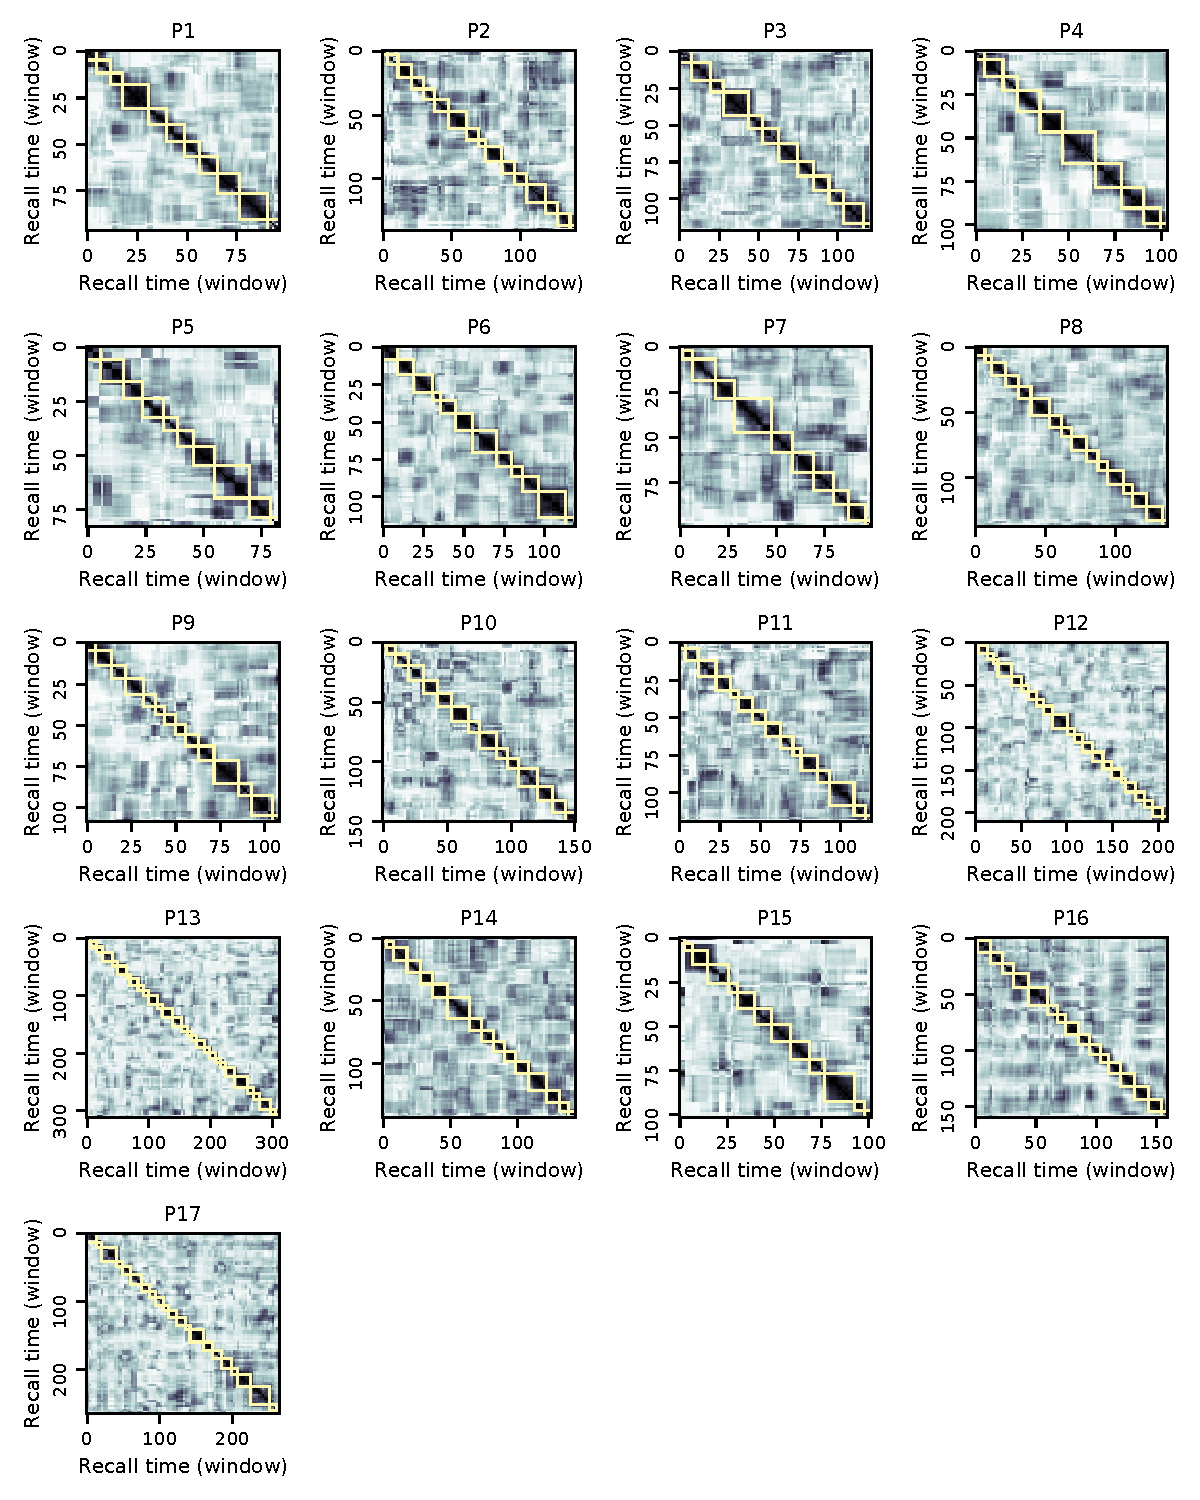
\includegraphics[width=\textwidth]{figs/corrmats}
\caption{\small \textbf{Recall trajectory temporal correlation matrices and event segmentation fits.} Each panel is in the same format as Figure~2E in the main text.  The yellow boxes indicate HMM-identified event boundaries.}
\label{fig:corrmats}
\end{figure}

\begin{figure}[p!]
\centering
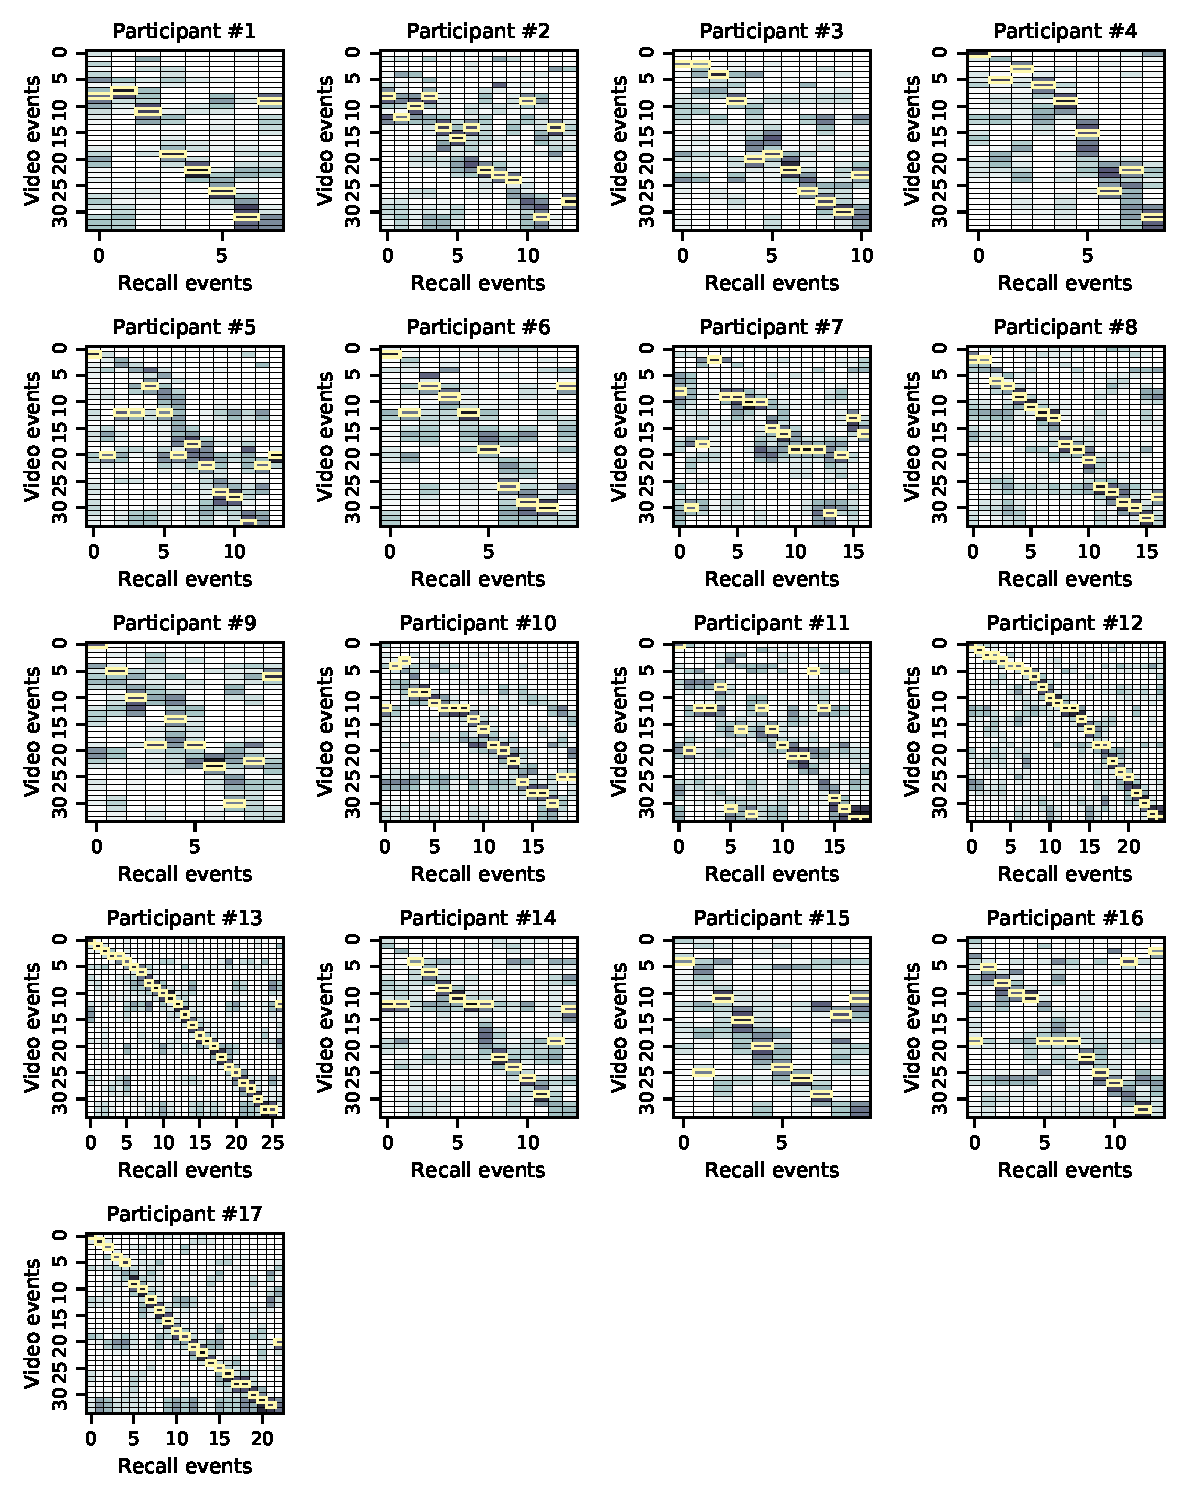
\includegraphics[width=\textwidth]{figs/matchmats}
\caption{\small \textbf{Video-recall event correlation matrices.}  Each panel is in the same format as Figure~2G in the main text.  The yellow boxes mark the maximum correlation in each column.}
\label{fig:matchmats}
\end{figure}

\begin{figure}[p!]
\centering
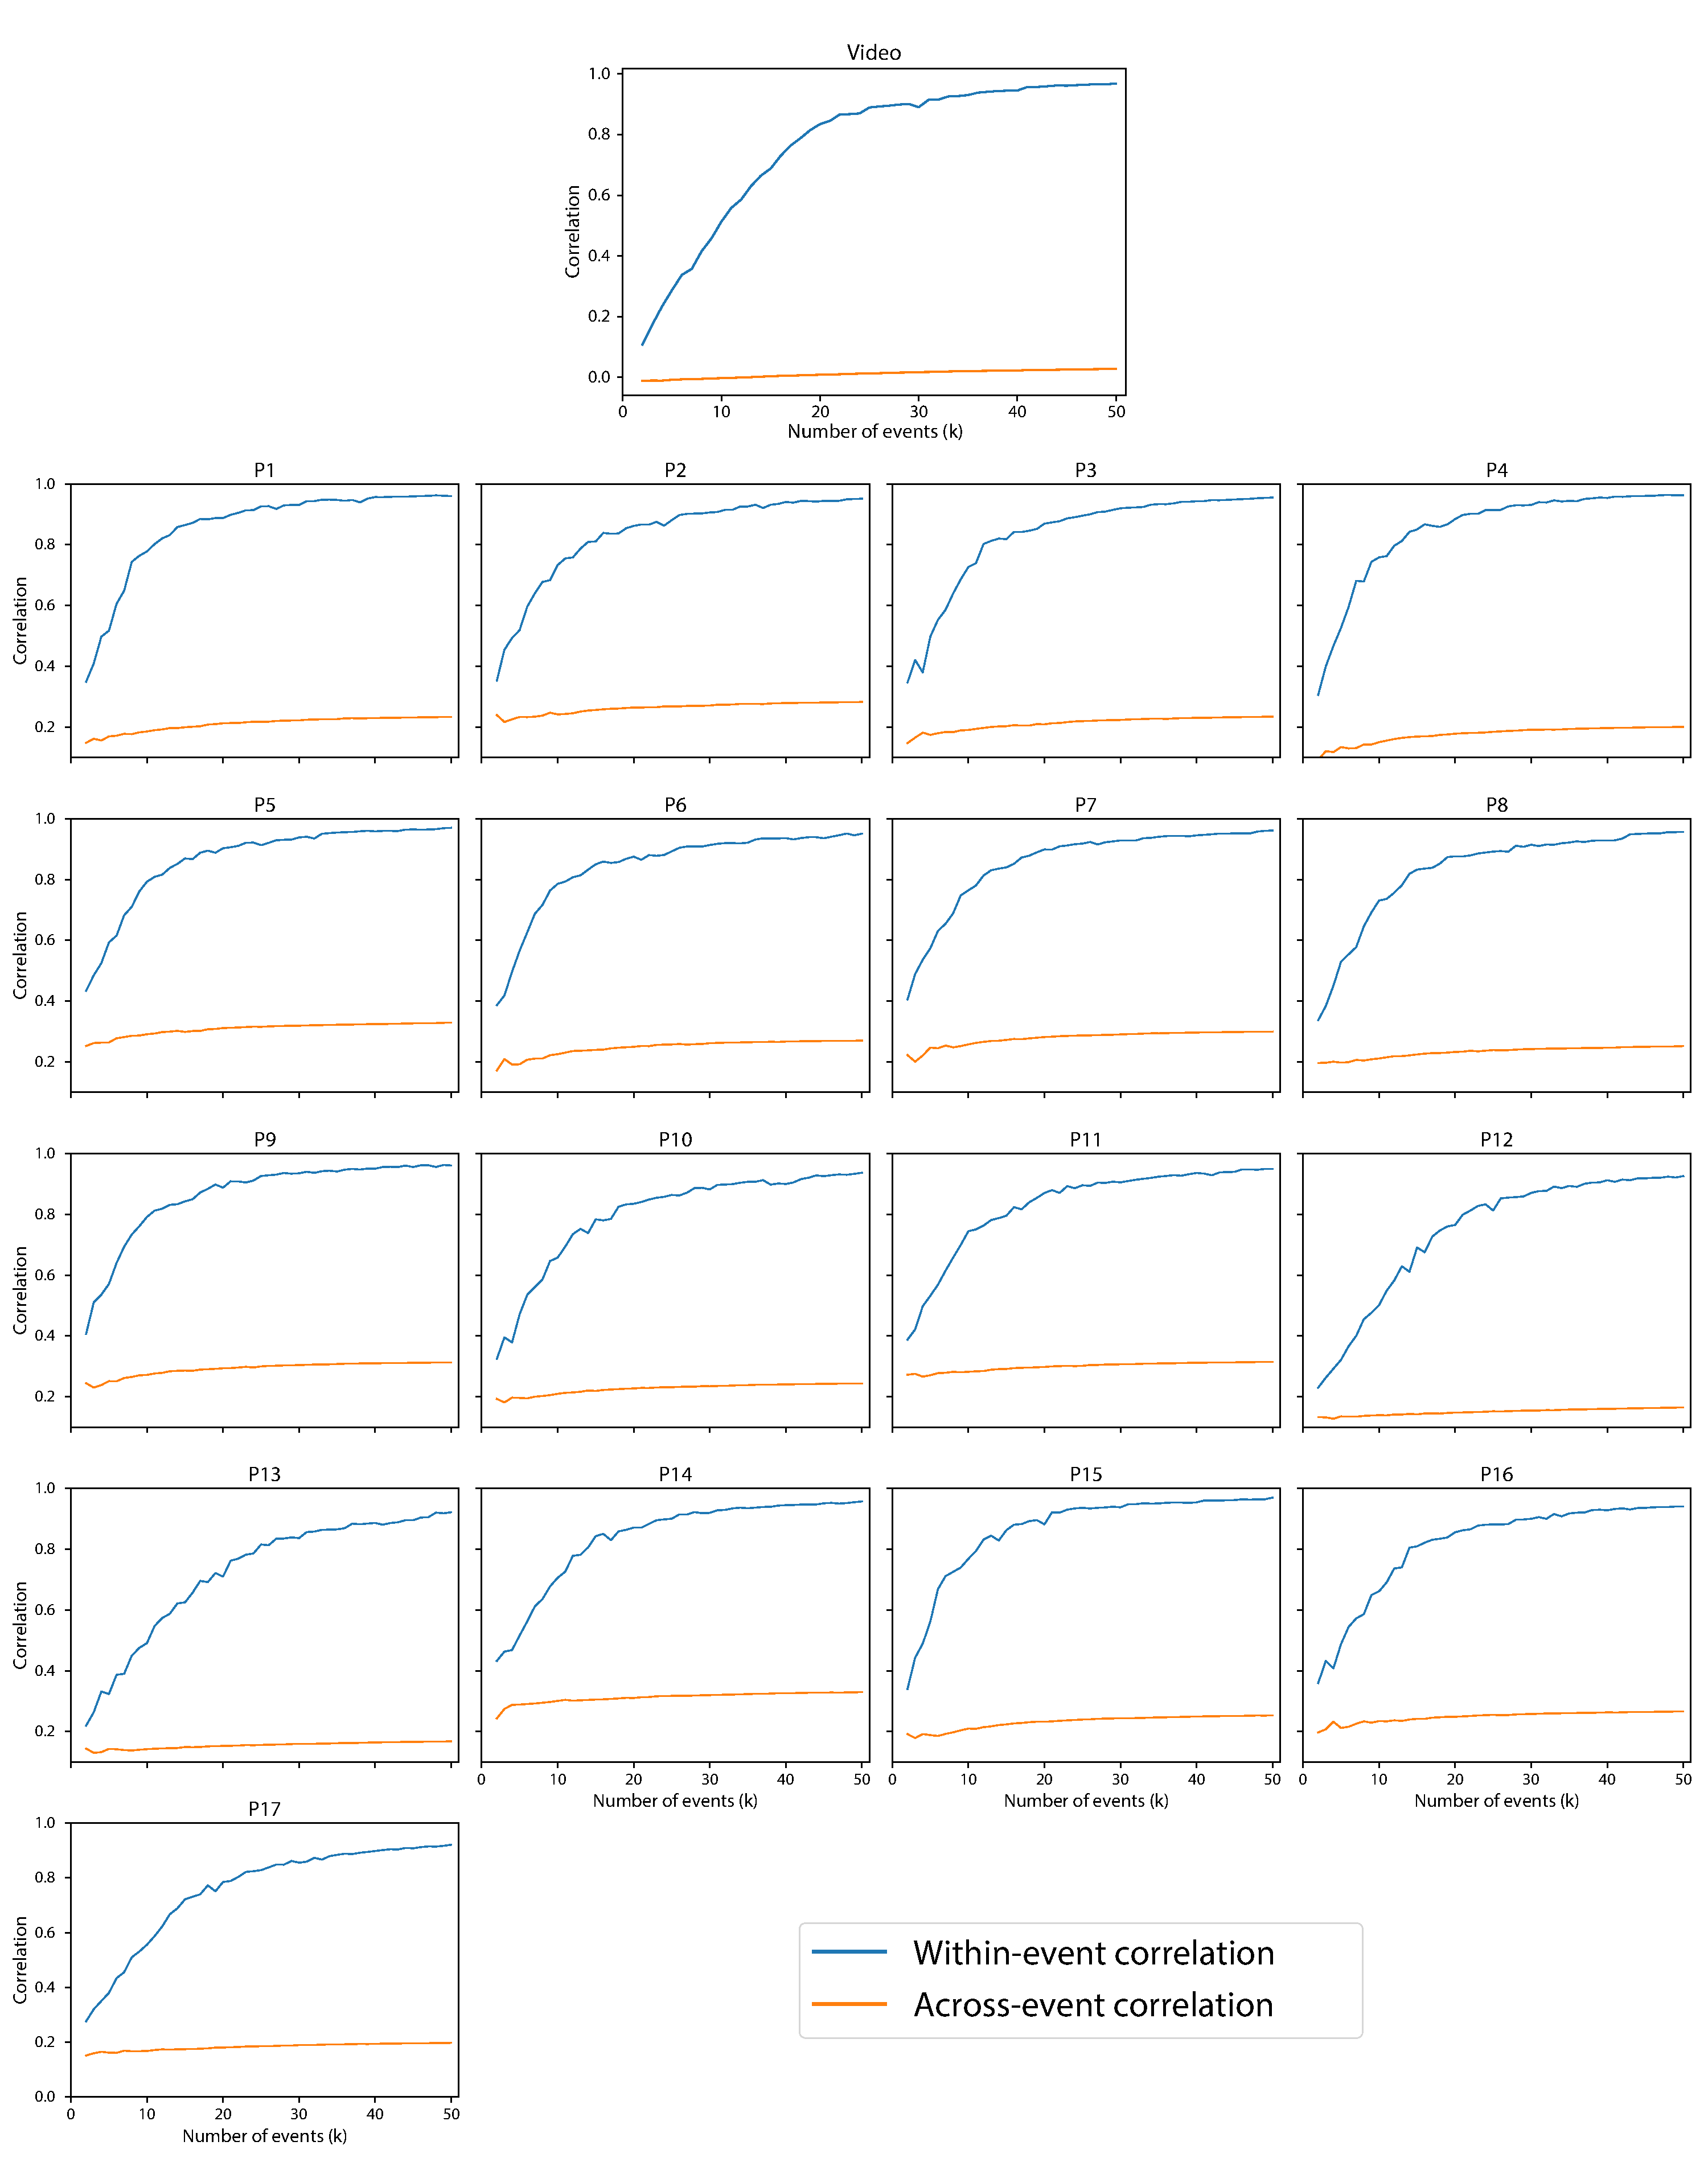
\includegraphics[width=.9\textwidth]{figs/k_corrs}
\caption{\small \textbf{Within- and across-event correlations as a function of $K$.}  As part of the event-segmentation procedure, we searched over a range of possible $K$-values [2,50] (i.e., number of events) for the video and each recall topic trajectory, separately.  For each $K$, we used an HMM to segment the trajectory into $K$-events. We then computed the average correlation between topic vectors at timepoints within the same event, and the average correlation between topic vectors at timepoints across different events.}
\label{fig:k_corrs}
\end{figure}

\begin{figure}[p!]
\centering
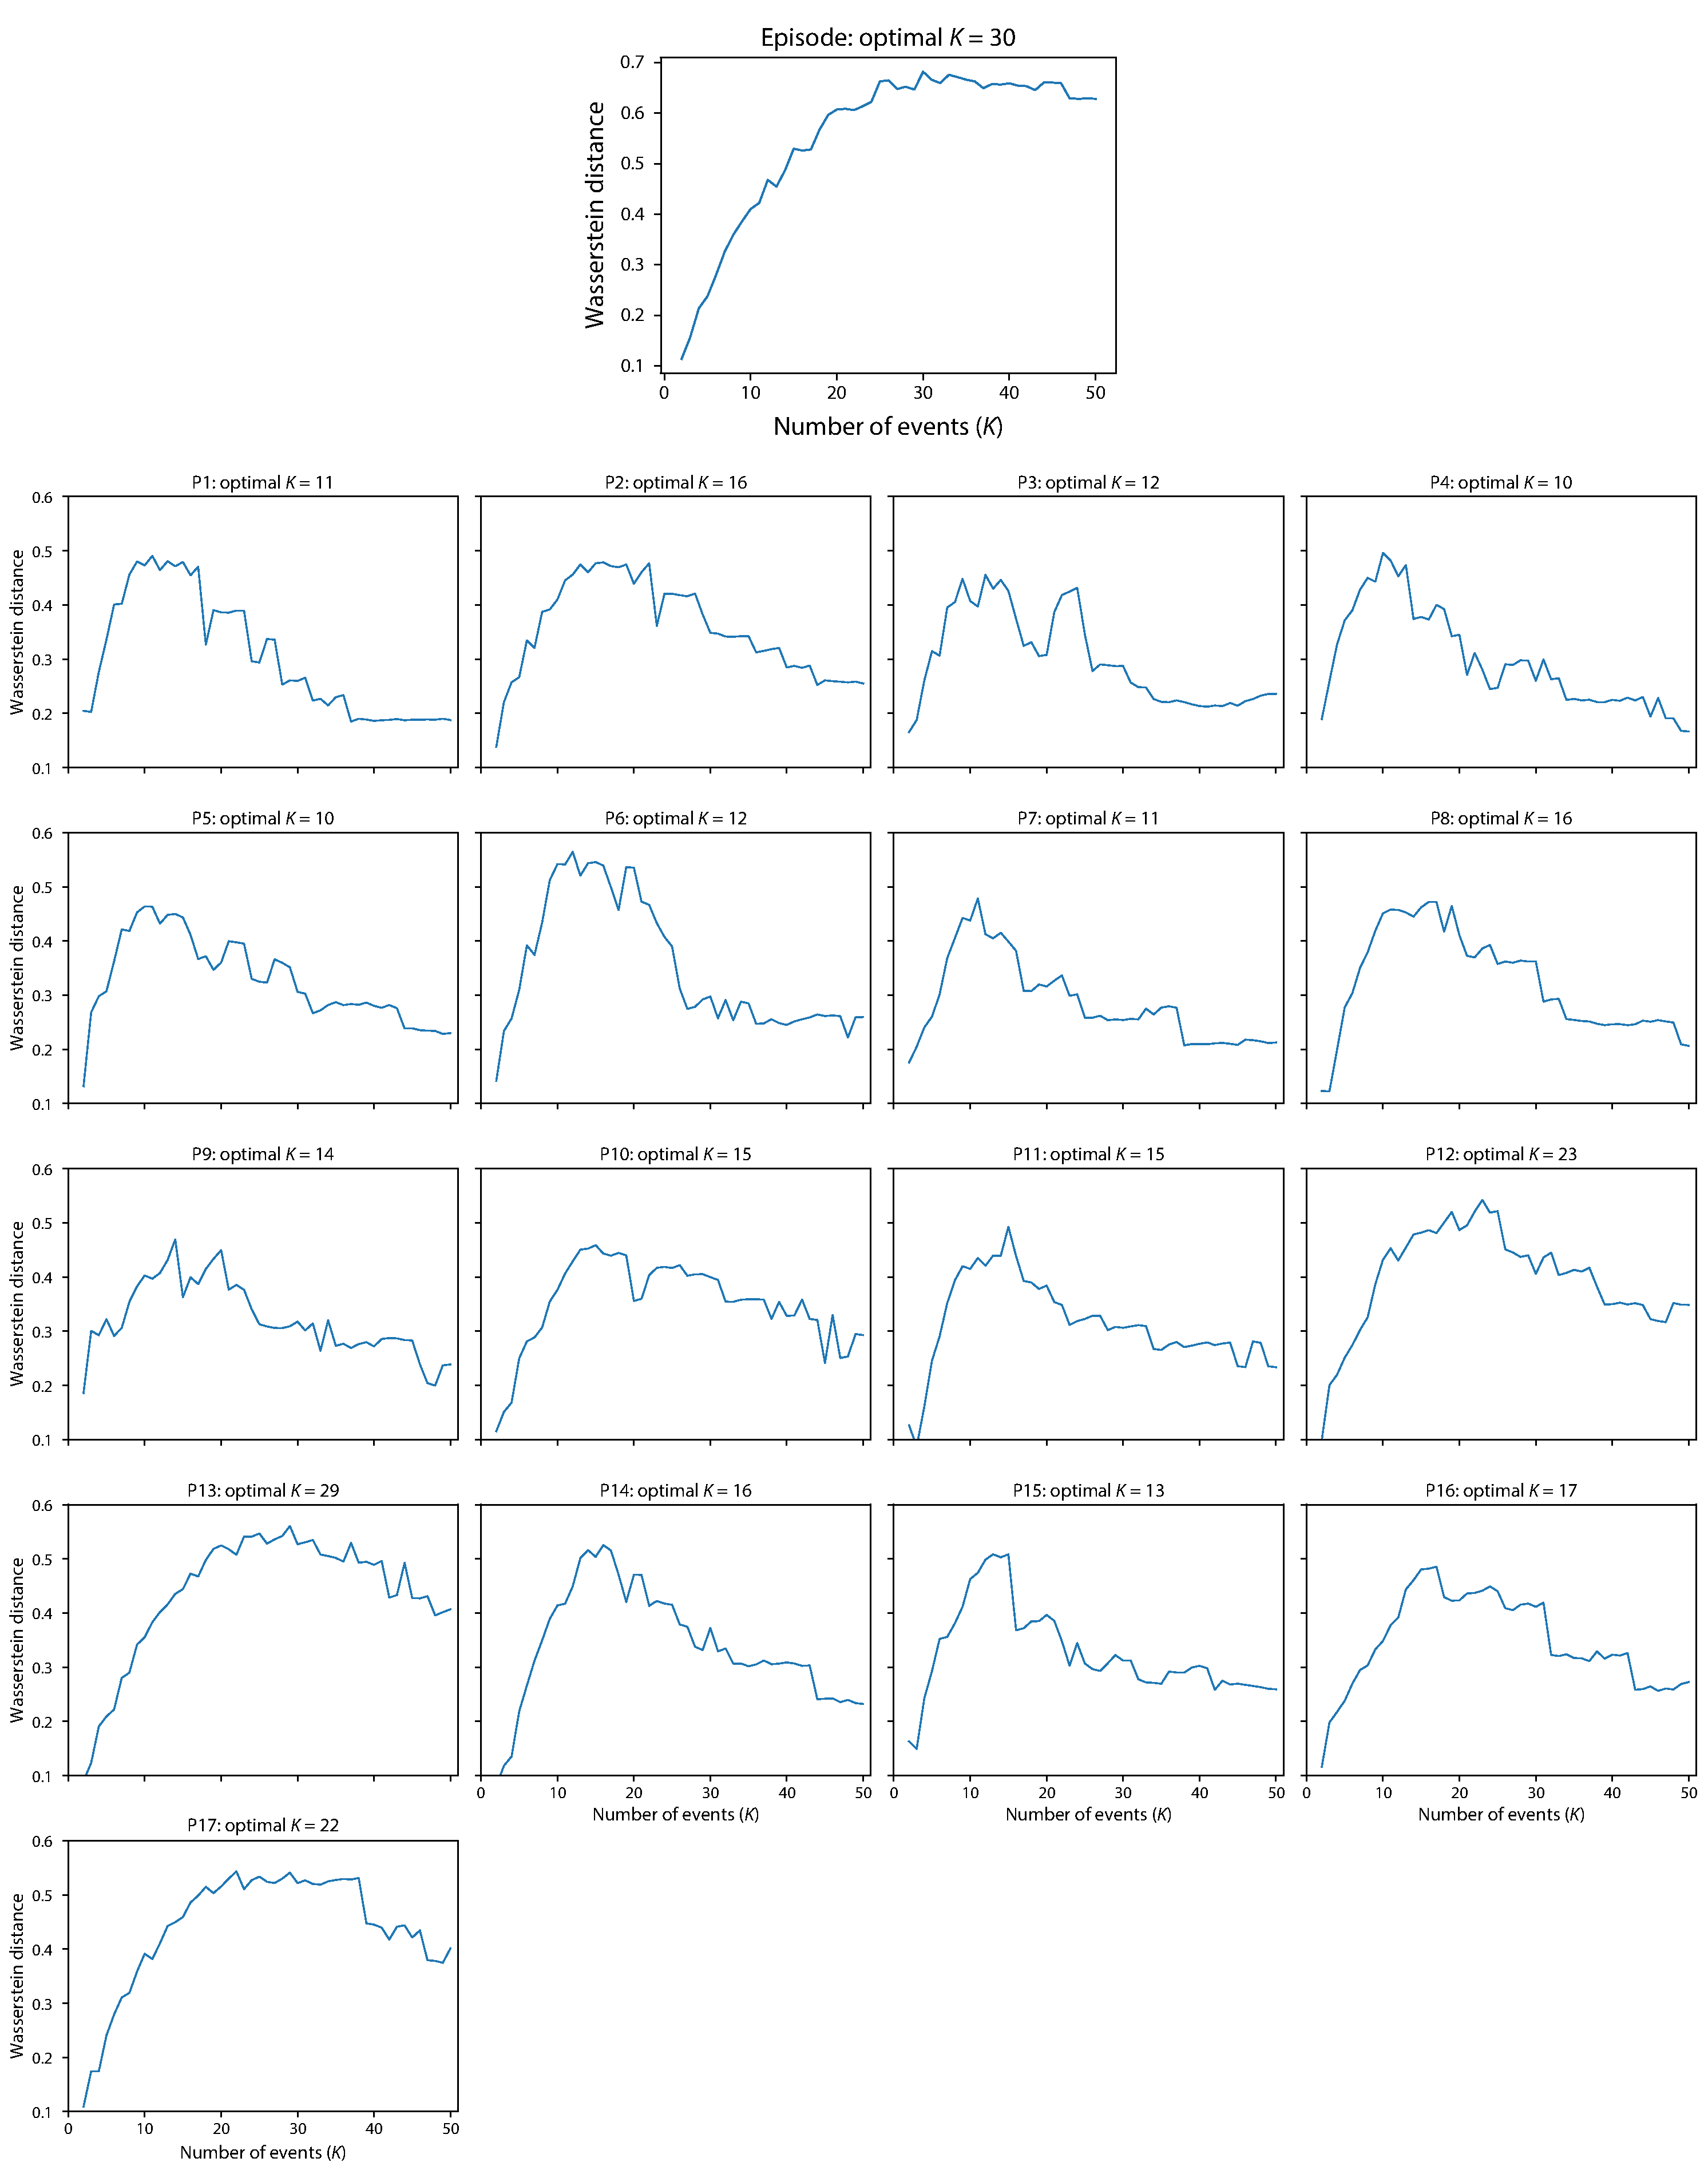
\includegraphics[width=.9\textwidth]{figs/k_optimization}
\caption{\small \textbf{Video and recall trajectory $K$-optimization functions.}  We selected the optimal $K$-value for the video and each recall trajectory, using the formula described in \textit{Methods}. This computation resulted in a curve for each trajectory, describing the regularized ratio of the average within-event topic vector correlation to the average across-event topic vector correlation, as a function of $K$.}
\label{fig:k_optimization}
\end{figure}

\begin{figure}[p!]
\centering
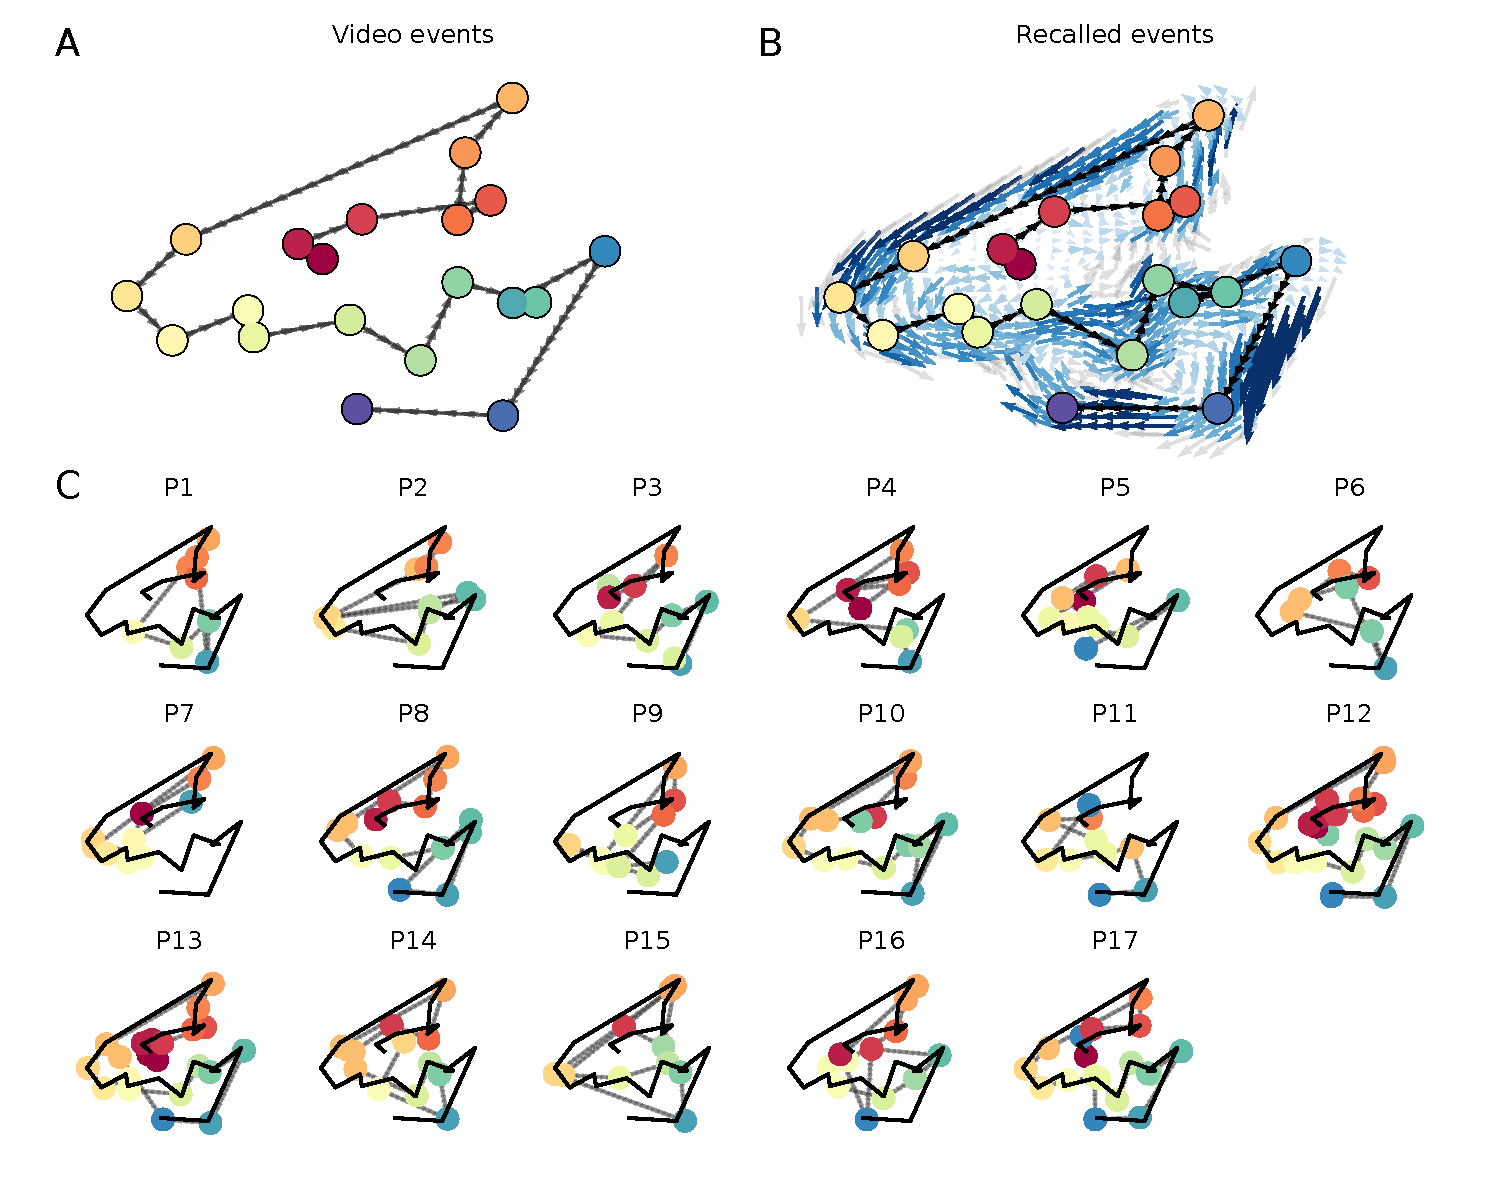
\includegraphics[width=\textwidth]{figs/trajectory_wasserstein}
\caption{\small \textbf{Trajectories using Wasserstein distance for choosing $K$.}  We replicated the trajectory analysis using Wasserstein distance, a parameter-free procedure for choosing $K$. Overall, the pattern of findings is quite similar to our main approach, but resulted in a smaller number of events.}
\label{fig:trajectory_wasserstein}
\end{figure}
  
\

\newpage
\renewcommand{\refname}{Supplemental references}
\bibliography{memlab}


\end{document}
